
%%%%%%%%%%%%%%%%%%%%%%%%%%%%%%%%%%%%%%%%%%%%%%%%%%%%%%%%%%%%%%%%%
%%%%%%%%%%%%%%%%%%%%%%%%%%%%%%%%%%%%%%%%%%%%%%%%%%%%%%%%%%%%%%%%%
\section{Introduction}
%%%%%%%%%%%%%%%%%%%%%%%%%%%%%%%%%%%%%%%%%%%%%%%%%%%%%%%%%%%%%%%%%
%%%%%%%%%%%%%%%%%%%%%%%%%%%%%%%%%%%%%%%%%%%%%%%%%%%%%%%%%%%%%%%%%
This manual is intended as a practical guide on how to obtain input parameters sensitivities and apply optimization strategies in B2.5 thanks to Algorithmic Differentiation (AD), therefore only \textit{using} the already available AD code. If one is interested in \textit{producing} new AD code, please see the ``Expert'' section \ref{cha:ad_expert}.

The user is invited to read the literature concerning AD for a more detailed theoretical background of this method, for example \cite{griewank}. The reference paper for AD on SOLPS-ITER is \cite{carlijcp}.
This particular application of AD makes use of the tool Tapenade \cite{tapenade}, which is available at \cite{tapesite}. Tapenade is a so-called source transformation AD tool, which means it will analyze the B2.5 source files and produce a new set of source files containing the derivative information. However, other AD tools are available, see for example the list in \cite{autodiff}, but they have not been tested on B2.5 so far and this manual might not be applicable to them.\\

The user must be aware that the AD differentiated code, available in \\
{\tt B2.5/src/differentiation/tangent} and
{\tt B2.5/src/differentiation/adjoint},\\
is not 100\% consistent with the current B2.5 code. The AD code will only be made consistent with the \textit{\textbf{release-ad}} branch/tag, when B2.5 will be re-differentiated and the AD files updated accordingly.

An additional caveat must be known by the user: this manual version and the procedure here described are valid and have been proven to work with specific Tapenade and SOLPS-ITER versions. New Tapenade releases and SOLPS-ITER development can make some of the procedure below obsolete or require modifications. Therefore, here are listed the git hash of both SOLPS-ITER and B2.5, and the Tapenade version that have been verified to work with this manual version:
\begin{description}
	\item{SOLPS-ITER} \href{https://git.iter.org/projects/BND/repos/solps-iter/commits/6d4ad74aa97fdd71df4b1bc008623603e0af3d78}{6d4ad74aa97}
	\item{B2.5} \href{https://git.iter.org/projects/BND/repos/b2.5/commits/3eabeb0698f9894e72e8ee832b09f8dbd07a1083}{3eabeb0698f}
	\item{Tapenade} \href{https://gitlab.inria.fr/tapenade/tapenade/-/commit/686e29d1a492ce72f4f7f61d94a47066695c9da8}{3.16-v2-120-g686e29d1a}
\end{description}


%%%%%%%%%%%%%%%%%%%%%%%%%%%%%%%%%%%%%%%%%%%%%%%%%%%%%%%%%%%%%%%%%
%%%%%%%%%%%%%%%%%%%%%%%%%%%%%%%%%%%%%%%%%%%%%%%%%%%%%%%%%%%%%%%%%
\section{Definition of the cost function}\label{sec:cost_fun}
%%%%%%%%%%%%%%%%%%%%%%%%%%%%%%%%%%%%%%%%%%%%%%%%%%%%%%%%%%%%%%%%%
%%%%%%%%%%%%%%%%%%%%%%%%%%%%%%%%%%%%%%%%%%%%%%%%%%%%%%%%%%%%%%%%%

Before calculating derivatives, the user first has to think which kind of cost function he is interested in. There are pre-defined cost functions already available within B2.5, defined in the subroutine {\tt b2usr\_cost\_function} and based on weighted least-squares and Bayesian Maximum A Posterior (MAP) frameworks described in \cite{carlpet21}.

	%%%%%%%%%%%%%%%%%%%%%%%%%%%%%%%%%%%%%%%%%%%%%%%%%%%%%%%%%%%%%%%%%
	\subsection{Regression cost function}
	%%%%%%%%%%%%%%%%%%%%%%%%%%%%%%%%%%%%%%%%%%%%%%%%%%%%%%%%%%%%%%%%%
	The nonlinear regression, weighted least-squares, cost function reads:

	\begin{equation} \label{regression0}
		\hat{\mathcal{J}}(\theta)=\sum_{l} \sum_{q} \frac{1}{\Omega_l} \int_{\Omega_l} \left(\frac{w_{l,q}}{\bar{q_l}^2} \frac{\left(q(\theta) - q^{\mathrm{EXP}}  \right)^2}{2} \right) \mathrm{d}\Omega.
	\end{equation}

	In Eq. \ref{regression0} $q$ indicates a general plasma quantity like density, temperature, etc., while $\theta$ indicates the set of input parameters (transport coefficients, boundary conditions, etc.), which one will eventually want to optimize. Furthermore, summation over $l$ indicates different spacial locations, for example OMP or target, while summation over $q$ indicates different state variables, for example plasma density $n_e$ or electron temperature $T_e$. The superscript \textit{EXP} indicates the experimental measurement.  $\Omega_l$ is the domain over which the integration is performed and $w_{l,q}$ are weighting factors. Finally, $\bar{q_l}=1/\Omega_l\int_{\Omega_l} q^{\mathrm{EXP}}\mathrm{d}\Omega$ is the average experimental value of $q$ over domain $\Omega_l$ used to normalize the terms in the cost function. The integral in Eq. \ref{regression0} is actually approximated as a discrete sum as indicate here below:
	\begin{equation} \label{regression}
		\hat{\mathcal{J}}(\theta)=\sum_{l} \sum_{q} \frac{1}{\Omega_l} \frac{w_{l,q}}{\bar{q_l}^2} \sum_{\Omega_{l,i}} \left( \frac{\left(q_i(\theta) - q_i^{\mathrm{EXP}}  \right)^2}{2} \right) \Omega_{l,i},
	\end{equation}
	where now the index $i$ refers to the discrete point in the sum. Such discrete points are the radial points specified by the experimental data, onto which the SOLPS-ITER quantities are interpolated.

	%%%%%%%%%%%%%%%%%%%%%%%%%%%%%%%%%%%%%%%%%%%%%%%%%%%%%%%%%%%%%%%%%
	\subsection{MAP cost function}
	%%%%%%%%%%%%%%%%%%%%%%%%%%%%%%%%%%%%%%%%%%%%%%%%%%%%%%%%%%%%%%%%%
	For a MAP estimation, the following cost function is employed:
	\begin{equation}\label{mapcost}
		\hat{\mathcal{J}}(\theta)=-\log\left[\mathcal{L}(\mathcal{D}\vert\theta)\pi(\theta)\right],
	\end{equation}
	where $\mathcal{D}$ is the experimental data set available for the analysis, of which $q^{\mathrm{EXP}}$ is a specific measurement. In Eq. \ref{mapcost} $\mathcal{L}(\mathcal{D}\vert \theta)$ is the likelihood function and $\pi(\theta)$ the prior distribution.

	The prior distribution $\pi(\theta)$ can be chosen by the user, and currently available options are uniform distributions (i.e. $\pi(\theta_i)=1.0$), or Gaussian priors $\frac{2}{\sigma_{\theta,i}\sqrt{(2\pi)}} \exp{\left[-\frac{1}{2} \frac{\left( \theta_i -\mu_{\theta_i}\right)^2}{\sigma_{\theta,i}^2} \right]}$, where $i$ indicates the specific element in the vector of control variables $\theta$, and $\mu_{\theta_i}$ and $\sigma_{\theta,i}$ are respectively the mean and standard deviation associated with the Gaussian for variable $\theta_i$.

	The likelihood function $\mathcal{L}(\mathcal{D}\vert \theta)$ is currently available as a Gaussian distribution, while other types will be implemented in future. The Gaussian likelihood for a quantity $q$ at a specific spatial location $\Omega_l$ takes the form
	\begin{equation}\label{likelihood}
		\mathcal{L}(\mathcal{D}\vert\theta)=\frac{1}{\sqrt{(2\pi)^{N_\mathcal{D}}\det\Sigma}} \exp{\left(-\frac{1}{2}z^T\Sigma^{-1}z \right)},
	\end{equation}
	where $z=q^{EXP}-q(\theta)-\mu$, $\Sigma$ is the covariance matrix and $N_\mathcal{D}$ is the number of data points $q^{EXP}$ for this specific quantity at this specific location $\Omega_l$. $\mu$ is the mean of the Gaussian distribution (not a tunable parameter at the moment). The covariance matrix is a diagonal matrix with $\Sigma_{ii}=\sigma_{q,l}^2$, if an absolute error is assumed in the likelihood. If instead the likelihood models a relative, instead of an absolute error, the diagonal elements of $\Sigma$ take the form $\Sigma_{ii}=\sigma_i^2=(\sigma_{q,l} q_i^{\mathrm{EXP}})^2$, with $\sigma_{q,l}$ a constant standard deviation. Note that in both cases $\sigma_{q,l}$ is the standard deviation associated with this specific quantity $q$ at this location $\Omega_l$.

	Whenever data is available at multiple locations (OMP, targets,...) and for multiple quantities (density, temperature,...), the total likelihood simply becomes the multiplication of the likelihood for each quantity at each spatial location, each of them with their specific standard deviation.

	%%%%%%%%%%%%%%%%%%%%%%%%%%%%%%%%%%%%%%%%%%%%%%%%%%%%%%%%%%%%%%%%%
	\subsection{How to specify the cost function in B2.5}
	%%%%%%%%%%%%%%%%%%%%%%%%%%%%%%%%%%%%%%%%%%%%%%%%%%%%%%%%%%%%%%%%%
	The user can select one of these cost functions through the input file {\tt b2.user.parameters}. To do so, it is needed to specify the following parameters, contained in the {\tt user} namelist, which are similar to the boundary condition specification. An up-to-date list is also available in \ref{lis:b2cdcn}.
	\begin{description}
		\item[NCF]\index{NCF} {\tt integer}, number of cost functions ({\tt icf = 1, NCF}). ({\tt DEFAULT = 0}).

		\item[CFTYPE] \index{CFTYPE} {\tt integer array, length NCF}, specifies the type of cost function for index {\tt icf}. ({\tt DEFAULT = -1}). Available options are:
		\begin{description}
			\item[0] Sum of weighted least squares cost functions. {\tt CFSTART, CFEND} indicate over which {\tt icf} indexes the cost functions are to be summed (valid cost function to be summed are types 1-3 and 7-9)

			\item[1]  Weighted least squares, on the desired CVs, of calculated electron density and experimental values read from file, normalized with average experimental value  (units must be $10^{19}m^{-3}$)

			\item[2] Weighted least squares, on the desired CVs, of calculated electron temperature and values read from file, normalized with average experimental value (units must be eV)

			\item[3] Weighted least squares, on the desired CVs, of calculated ion temperature and values read from file, normalized with average experimental value (units must be eV)

			\item[4] Maximum electron temperature on the desired CVs (output in eV)

			\item[5] Maximum heat flux on the desired FCs (output in W)

			\item[6] Bayesian MAP cost function (see \cite{carlpet21}). {\tt CFSTART, CFEND} indicate over which {\tt icf} indexes the cost functions are to be summed (valid cost function to be summed are types are 1-3 and 7-9)

			\item[7] Weighted least squares, on the desired CVs, of calculated electron density radial gradient and experimental values read from file, normalized with average experimental value  (units must be $10^{19}m^{-4}$)

			\item[8] Weighted least squares, on the desired CVs, of calculated electron temperature radial gradient and values read from file, normalized with average experimental value (units must be $eV/m$)

			\item[9] Weighted least squares, on the desired CVs, of calculated ion temperature radial gradient and values read from file, normalized with average experimental value (units must be $eV/m$)
		\end{description}

		\item[CFDEF] \index{CFDEF} {\tt integer array, length NCF}, indicates how the domain of cost function {\tt ifc} is specified. ({\tt DEFAULT = 0}). Valid options are:
		\begin{description}
			\item[1] The cost function is defined on the OMP, using the {\tt rzomp} array. In this case {\tt CFSTART,CFEND} are not necessary and ignored.

			\item[2] The cost function is defined using the FC labels specified in {\tt CFSTART,CFEND}. Cost functions requiring CVs or FCs can both be defined in this way.

			\item[3] The cost function is defined using the CV labels specified in {\tt CFSTART,CFEND}. Only cost functions requiring CVs can be defined in this way.

			\item[4] The cost function is defined using the {\tt CF\_REG} and {\tt CF\_REGP} arrays. Cost functions requiring CVs or FCs can both be defined in this way.
		\end{description}

		\item[CFSTART,CFEND] \index{CFSTART,CFEND} {\tt integer arrays, length NCF}, specify the starting/ending, face (FC) label {\tt fcLbl} or control volume (CV) label {\tt cvLbl} where the cost function {\tt icf} will be evaluated. For {\tt CFTYPE = 0} and {\tt CFTYPE = 6} they instead identify which cost functions will be summed together. ({\tt DEFAULT = 0}).

		\item[CF\_REGP] \index{CF\_REGP} {\tt integer array, length (NCF, 2)}. Points for each cost function to the first index in the {\tt CF\_REG} list, and its number of items. ({\tt DEFAULT = 0}).

		\item[CF\_REG] \index{CF\_REG} {\tt integer array, length mxnCf}. Listing for each cost function the corresponding domain CVs or FCs. WARNING! No attempt is made to check if these CVs or FCs are connected, sorted or even available in the current geometry: it is up to the user to make sure the list is correct. ({\tt DEFAULT = 0}).

		\item[CFWEIGHT] \index{CFWEIGHT} {\tt real array, length NCF}. Multipliers to re-scale each cost function separately, $w_{l,q}$ in Eq. \ref{regression}. ({\tt DEFAULT = 1.0}).

		\item[MapToOMP] \index{MapToOMP} {\tt logical array, length NCF}. Indicates if cost function icf is to be re-mapped to the OMP, according to CFTYPE. Warning! The mapping is a rigid traslation of the data to the OMP and is safe to work only for non-extended grids and for cost functions defined on the same number of elements as the OMP list.  ({\tt DEFAULT = .FALSE.}).

		\item[NSIGMA] \index{NSIGMA}  {\tt integer}, number of standard deviation variables used for Bayesian MAP cost function (normally this should be equal to the number of cost functions summed for CFTYPE = 6, i.e. one for each variable on each domain) ({\tt isigma = 1, NSIGMA}). ({\tt DEFAULT = 0}).

		\item[SIGMA] \index{SIGMA}  {\tt real array, length NSIGMA}. Value of the standard deviation $\sigma$ in the likelihood function. For absolute STD the units are the same as the experimental data used for the cost function it refers to. ({\tt DEFAULT = 0.0}).

		\item[SCALE\_SIGMA] \index{SCALE\_SIGMA} {\tt logical array, length NSIGMA}, indicates if {\tt SIGMA(isigma)} is intended as relative standard deviation ({\tt SCALE\_SIGMA(isigma)=.TRUE.}) or absolute ({\tt SCALE\_SIGMA(isigma)=.FALSE.}).  ({\tt DEFAULT = .TRUE.}).

		\item[PRIOR\_TYPE] \index{PRIOR\_TYPE}  {\tt integer arrays, length NNVAR}. Defines the type of prior distribution for each parameter for the MAP cost function. ({\tt DEFAULT = -1}). Possible values are
		\begin{description}
			\item[0] Uniform distribution.

			\item[1] Uninformative, proper, Gaussian prior.
		\end{description}

		\item[PRIOR\_PAR] \index{PRIOR\_PAR} {\tt real array, length (NNVAR,2)}. Indicates parameters for the prior distributions. For ({\tt DEFAULT = -1.0}). For {\tt PRIOR\_TYPE}
		\begin{description}
			\item[0] Not used

			\item[1] {\tt PRIOR\_TYPE(ii,1)} indicates the mean $\mu_{\theta_i}$ of and {\tt PRIOR\_TYPE(ii,2)} indicates the standard deviation $\sigma_{\theta,i}$ of the Gaussian distribution
		\end{description}

		\item[PRIOR\_RANGE] \index{PRIOR\_RANGE} {\tt real array, length (NNVAR,2)}. Indicates the valid range for the prior distributions, outside of which the program will return an infinite cost function value. {\tt PRIOR\_RANGE(:,1)} sets the lower range and {\tt PRIOR\_RANGE(:,2)} sets the upper range. ({\tt DEFAULT = $\pm 10p_{\infty}$}, where $p_{\infty}$ is a parameter is currently set to $10^{30}$)

	\end{description}


	If experimental data needs to be read (e.g. for cost functions 1-3, 7-9), these must be available in a file named {\tt cfi.dat}, with {\tt i} corresponding to the cost function index  {\tt icf} (not the type!). Within the file, the user has to specify two columns of the same length, the first containing the radial distance from the separatrix (in units of m), and the second containing the data value (units described above). The calculated B2.5 quantities are then interpolated onto the specified radial domain, while no extrapolation is allowed.\\

	Labels for FCs ({\tt fcLbl}) and CVs ({\tt cvLbl}) can be specified within {\tt b2fgmtry}. Boundary FCs already have a label assigned to impose boundary conditions, therefore for cost functions defined at the targets, these labels can readily be used.\\

	Dedicated internal mapping arrays have been additionally defined in {\tt b2us\_map} to collect the FCs and CVs on which cost functions are defined:
	\begin{description}

		\item[cfRegP] \index{cfRegP} {\tt integer array, length (NCF, 2)}. pointing for each cost function to the first index in the {\tt cfReg} list, and its number of elements


		\item[cfReg] \index{cfReg} {\tt integer array, length mxnCf}. listing for each cost function the corresponding domain cells or faces

		\item[cfOnCv] \index{cfOnCv} {\tt logical array, length nCf}. Logical to indicate whether a cf domain is on CV (true) or FC (false)

		\item[cfFcOr] \index{cfFcOr} {\tt real array, length nCf}. Multiplier to indicate whether outward normal coincides with the face normal (1.0) or not (-1.0)
	\end{description}

	Cost functions requiring cell-centered quantities like density or temperature can be correctly defined also using FC labels, since the lowest numbered internal CV belonging to each face will be mapped.\\

	Finally, the user can specify additional ad-hoc cost functions for own purposes, modifying the source file: \\ {\tt B2.5/src/user/b2usr\_cost\_function.F},\\
	after which re-differentiation is needed (see Expert mode \ref{cha:ad_expert})

	%%%%%%%%%%%%%%%%%%%%%%%%%%%%%%%%%%%%%%%%%%%%%%%%%%%%%%%%%%%%%%%%%
	\subsection{Example of cost function file}\label{sec:cfexample}
	%%%%%%%%%%%%%%%%%%%%%%%%%%%%%%%%%%%%%%%%%%%%%%%%%%%%%%%%%%%%%%%%%
	\textbf{Regression cost function}\\
	Let's take as an example the case of a cost function including electron density, electron temperature and ion temperature at the OMP, and electron density and temperature at the outer target. These have to be summed together in a weighted least-squares approach. Therefore, in {\tt b2.user.parameters} one needs to specify:\\

	{\tt NCF = 6}

	{\tt CFTYPE = 0, 1, 2, 3, 1, 2}\\

	where the {\tt 0} indicates the sum of the cost functions, {\tt 1} indicates electron density, {\tt 2} electron temperature and {\tt 3} ion temperature. Suppose the face label of the outer target is {\tt -34}, then to define the cost function there and at the OMP one needs:\\

	{\tt CFSTART = 2, 0, 0, 0, -34, -34,}

	{\tt CFEND =   6, 0,  0, 0, -34, -34,}

	{\tt CFDEF =   0, 1,  1,  1, 2, 2,}\\

	where {\tt CFSTART(1)=2} and {\tt CFEND(1)=6} indicate the indexes of cost functions to be summed together (from 2 to 6).  {\tt CFSTART(2:4)=CFEND(2:4)=0} because these cost functions are defined on the OMP ({\tt CFDEF(2:4)=1}). Finally, the ones defined on the outer target use the FC label ({\tt CFDEF(2:4)=2}) number -34 and have thus {\tt CFSTART(5:6)=}{\tt CFEND(5:6)=-34}.


	Finally, the user still needs to provide experimental data for each of these cost functions, which should be saved in files named: {\tt cf2.dat}, for electron density at OMP; {\tt cf3.dat}, for electron temperature at OMP; {\tt cf4.dat}, for ion temperature at OMP; {\tt cf5.dat}, for electron density at target; {\tt cf6.dat} , for electron temperature at target.( Note the name numbering starts at 2 as this is the index of the first cost function actually needing to read data!)\\

	\textbf{MAP cost function}\\
	If the user is instead interested in using a Bayesian MAP cost function defined on the same domains and using the same quantities as above, then it is necessary to modify the first cost function type to have:\\

	{\tt CFTYPE = 6, 1, 2, 3, 1, 2}\\

	Furthermore, standard deviations needs to be specified for each of the five summed cost functions. Supposing for all OMP quantities a relative standard deviation of 10\%, and for target quantities an absolute standard deviation of $20^{18} m^{-3}$ for electron density and $5$ eV for electron temperature:\\

	{\tt NSIGMA = 5,}

	{\tt SIGMA =  0.1, 0.1, 0.1, 0.2, 5,}

	{\tt SCALE\_SIGMA = T, T, T, F, F,}\\

	where {\tt SIGMA(1:3) = 0.1} refer to the 10\% relative standard deviation for the OMP cost functions for which {\tt SCALE\_SIGMA(1:3) = T}; {\tt SIGMA(4) = 0.2} refers to the $20^{18} m^{-3}$ standard deviation for electron density (in units of $10^{19}m^{-3}$) in absolute form {\tt SCALE\_SIGMA(4) = F}; {\tt SIGMA(5) = 5.0} refers to the $5$ eV standard deviation for electron temperature in absolute form {\tt SCALE\_SIGMA(5) = F}.

	Suppose finally that a Gaussian prior distribution well describes the standard deviation for the OMP quantities, with zero mean and 10.0 standard deviation, while for the target quantities a uniform prior can be used. Then one must set:\\

	{\tt PRIOR\_TYPE = 1, 1, 1, 0, 0,}

	{\tt PRIOR\_PAR(1,1) = 0.0, 0.0, 0.0,}

	{\tt PRIOR\_PAR(1,2) = 10.0, 10.0, 10.0,}\\

	Finally, all these priors refer to a quantity (the standard deviation of the plasma density/temperature), which by definition must be a positive, nonzero number. Therefore the lower range of the priors must be adjusted to e.g.:\\

	{\tt PRIOR\_RANGE(1,1) = 1.0e-5, 1.0e-5, 1.0e-5, 1.0e-5, 1.0e-5,}


%%%%%%%%%%%%%%%%%%%%%%%%%%%%%%%%%%%%%%%%%%%%%%%%%%%%%%%%%%%%%%%%%
%%%%%%%%%%%%%%%%%%%%%%%%%%%%%%%%%%%%%%%%%%%%%%%%%%%%%%%%%%%%%%%%%
\section{Tangent AD mode}\label{sec:forwardAD}
%%%%%%%%%%%%%%%%%%%%%%%%%%%%%%%%%%%%%%%%%%%%%%%%%%%%%%%%%%%%%%%%%
%%%%%%%%%%%%%%%%%%%%%%%%%%%%%%%%%%%%%%%%%%%%%%%%%%%%%%%%%%%%%%%%%
The tangent (or forward) AD mode is the simplest one and allows the user to obtain simultaneously the gradient of all cost functions (outputs) with respect to a single input parameter. For details on the tangent mode the user is referred to \cite{griewank}. The tangent AD is also the first type of AD that has been applied successfully on B2.5 \cite{carlipsi}.\\
In tangent AD mode, the user can thus specify as many cost functions as desired, but the differentiation can be done with respect to only one input parameter. There is, however, the possibility to exploit the so-called vector AD mode, which allows to obtain the full Jacobian, i.e. the derivatives of all cost functions wrt multiple input parameters. The computational cost of such method will however increase proportionally to the number of input parameters, therefore one must think whether the adjoint AD mode can be more efficient, see section \ref{sec:adjointAd}. The tangent AD code currently available in B2.5 has been produced using such tangent vector mode.

	%%%%%%%%%%%%%%%%%%%%%%%%%%%%%%%%%%%%%%%%%%%%%%%%%%%%%%%%%%%%%%%%%
	\subsection{Code compilation}
	%%%%%%%%%%%%%%%%%%%%%%%%%%%%%%%%%%%%%%%%%%%%%%%%%%%%%%%%%%%%%%%%%
	To compile the tangent code make the objects and dependencies list in the standard way in {\tt \$SOLPSTOP}:\\
	{\tt \$ gmake listobj depend}\\
	Then compile with:\\
	{\tt \$ gmake b25\_tgt}\\

	This way a new executable called {\tt b2mn\_d} will be created in \\
	{\tt B2.5/builds/standalone.\${HOST\_NAME}.\${COMPILER}.tgt}.

	In case the {\tt debug} version is needed, it follows the standard {\tt SOLPS-ITER} rules which simply require to append {\tt \_debug} to the make targets.


	%%%%%%%%%%%%%%%%%%%%%%%%%%%%%%%%%%%%%%%%%%%%%%%%%%%%%%%%%%%%%%%%%
	\subsection{Code run}
	%%%%%%%%%%%%%%%%%%%%%%%%%%%%%%%%%%%%%%%%%%%%%%%%%%%%%%%%%%%%%%%%%
	Once the code has been successfully compiled, it can be run with the following command:\\

	{\tt \$ b2run -tgt b2mn > run.log}\\

	This code will converge the original B2.5 equations (also called the primal) and at the same time also the tangent equations (derivative of the original equations in tangent mode). By default, running this version of the code will calculate the derivative of ANY cost function wrt three basic parameters:
	\begin{itemize}
		\item {\tt parm\_dna(1)}: particle diffusion coefficient for species 1
		\item {\tt parm\_hce}:  electron heat diffusion coefficient
		\item {\tt parm\_hci(1)}: ion heat diffusion coefficient for species 1
	\end{itemize}

	The code will automatically print in run.log the value of the cost function(s) and their derivatives. To check it, simply do:\\

	{\tt \$ grep -i cost run.log}\\

	Users have other options to monitor the progress of the derived quantities:
	\begin{description}
		\item[cost\_function \$i] This script allows the user to plot the value of the cost function {\tt \$i} as a function of the iterations

		\item[cost\_function\_gradient \$i] This script allows the user to plot the value of the gradient of cost function {\tt \$i} as a function of the iterations

		\item[resall\_D\_diff] This script plots the evolution of the residuals of all the differentiated equations for D only cases

		\item[resco\_diff] This script plots the evolution of the residuals of the differentiated continuity equation

		\item[resmo\_diff] This script plots the evolution of the residuals of the diff'ed momentum equation

		\item[resrest\_diff] This script plots the evolution of the residuals of the diff'ed total momentum, ion energy, electron energy and potential equations

		\item[2dt\_diff] To be done if needed
	\end{description}

	%%%%%%%%%%%%%%%%%%%%%%%%%%%%%%%%%%%%%%%%%%%%%%%%%%%%%%%%%%%%%%%%%
	\subsection{Derivatives of more parameters}\label{sec:tanget_more}
	%%%%%%%%%%%%%%%%%%%%%%%%%%%%%%%%%%%%%%%%%%%%%%%%%%%%%%%%%%%%%%%%%
	If the derivative of any other coefficient is needed, then {\tt b2mn\_d.F90} in {\tt B2.5/src/differentiation/tangent} must be modified accordingly, as suggested by the commented example in the file itself, recalling that {\tt nbdirs} must be set to the desired number of independent variables.

	{\tt b2mod\_diffsizes.F} acts similarly to {\tt DIMENSIONS.F} and stores the maximum number of directions {\tt nbdirsmax} allowed, i.e. the maximum number of indpendent variables with respect to which one can calculate the derivative of the cost function. Increase nbdirsmax and recompile if needed.

	Current parameters for which derivative calculation is possible (default parameters):
	\begin{itemize}
		\item Transport coefficients: {\tt parm\_dna}, {\tt parm\_hce}, {\tt parm\_hci}, {\tt parm\_vsa}, {\tt parm\_sig}, {\tt parm\_alf }
		\item Radially-varying and ballooned transport coefficients: {\tt tdata}, {\tt b2tqna\_ballooning},\\ {\tt b2tqna\_ballooning\_rescale}
		\item Boundary conditions: {\tt enepar}, {\tt enipar}, {\tt conpar}, {\tt mompar}, {\tt potpar}, {\tt enkpar }
		\item Recycling coefficients: {\tt b2recyc }
		\item $\kappa$-model switches: {\tt keps\_cd}, {\tt b2sikt\_fac\_sheath}, {\tt b2sikt\_fac\_sheath\_core}, {\tt b2sikt\_fac\_diss}, {\tt b2sikt\_fac\_diss\_core}, {\tt b2tfhi\_fsigkt}, {\tt keps\_heat}, {\tt keps\_heat\_i}, {\tt keps\_sig}, {\tt keps\_alf}, {\tt keps\_visc}, {\tt keps\_dkt}, {\tt keps\_dzt}, {\tt keps\_shear}, {\tt b2sikt\_fac\_vis\_RS}, {\tt b2tfhi\_fflokt},\\ {\tt b2tfhi\_fconkt}, {\tt b2tfhi\_fflozt}, {\tt b2tfhi\_fconzt}, {\tt b2tfhi\_fkt\_hie}, {\tt b2tfhe\_vis\_kt }
		\item Reaction rates: {\tt rtlsa}, {\tt rtlra}, {\tt rtlcx}, {\tt rtlqa}
		\item Optimization parameters: {\tt sigma}, {\tt par\_opt\_phys}
	\end{itemize}



%%%%%%%%%%%%%%%%%%%%%%%%%%%%%%%%%%%%%%%%%%%%%%%%%%%%%%%%%%%%%%%%%
%%%%%%%%%%%%%%%%%%%%%%%%%%%%%%%%%%%%%%%%%%%%%%%%%%%%%%%%%%%%%%%%%
\section{Adjoint AD mode}\label{sec:adjointAd}
%%%%%%%%%%%%%%%%%%%%%%%%%%%%%%%%%%%%%%%%%%%%%%%%%%%%%%%%%%%%%%%%%
%%%%%%%%%%%%%%%%%%%%%%%%%%%%%%%%%%%%%%%%%%%%%%%%%%%%%%%%%%%%%%%%%

The adjoint (or backward) AD mode allows the user to obtain the gradient of a single cost function with respect to all input parameters, at a cost which is around 5 times that of a standard B2.5 simulation. For details on the adjoint mode the user is referred to \cite{griewank}. The reference work for adjoint AD on B2.5 is \cite{carlijcp}.

While in principle adjoint vector mode exists and allows to retrieve the full Jacobian, this has not yet been deployed in SOLPS.


	%%%%%%%%%%%%%%%%%%%%%%%%%%%%%%%%%%%%%%%%%%%%%%%%%%%%%%%%%%%%%%%%%
	\subsection{Code compilation}
	%%%%%%%%%%%%%%%%%%%%%%%%%%%%%%%%%%%%%%%%%%%%%%%%%%%%%%%%%%%%%%%%%
	To compile the adjoint code make the objects and dependencies list in the standard way in {\tt \$SOLPSTOP}:\\
	{\tt \$ gmake listobj depend}\\
	Then compile with:\\
	{\tt \$ gmake b25\_adj}\\

	Similarly as for tangent AD, a new executable called {\tt b2mn\_b} will be created in \\
	{\tt B2.5/builds/standalone.\${HOST\_NAME}.\${COMPILER}.adj}.

	In case the {\tt debug} version is needed, it follows the standard {\tt SOLPS-ITER} rules which simply require to append {\tt \_debug} to the make targets.


	%%%%%%%%%%%%%%%%%%%%%%%%%%%%%%%%%%%%%%%%%%%%%%%%%%%%%%%%%%%%%%%%%
	\subsection{Code run}\label{sec:run_adj}
	%%%%%%%%%%%%%%%%%%%%%%%%%%%%%%%%%%%%%%%%%%%%%%%%%%%%%%%%%%%%%%%%%
	Once the code has been successfully compiled, it can be run with the following command:\\

	{\tt \$ b2run -adj b2mn > run.log}\\

	The adjoint code features a small difference wrt to the tangent in that it first converges the primal, and then converges the adjoint equations, keeping the converged primal state fixed, see \cite{carlijcp} and Figure \ref{fig_adjoint}. In this framework, there are two stopping criteria for both the primal and the adjoint iterations: either the maximum number of iterations set by {\tt b2mndr\_ntim} or a threshold for the maximum residual set by {\tt b2mndr\_res\_quit} (default {\tt 1e-7}). When either of the two is reached, the primal or adjoint iterations are stopped. The maximum residual is calculated for the primal as the maximum among the L1-norms of the residuals of the solved equations (variables {\tt aresco, aresmo, etc} already available in the code). For the adjoint, this residual is instead calculated as the maximum of the quantities:
	\begin{equation}\label{res}
		R_q = \frac{\sqrt{\sum_{i} (\bar{q}(i) -\bar{q}_0(i))^2}}{\sqrt{\sum_{i} \bar{q}(i)^2}}
	\end{equation}
	where $\bar{q}$ indicates an adjoint state variable (density, velocity, electron temperature, etc.), $\bar{q}_0$ indicates the same adjoint state variable at the previous iteration, and the sum is done over each cell $i$ of the domain.

	\begin{figure}[h]
		\begin{center}
			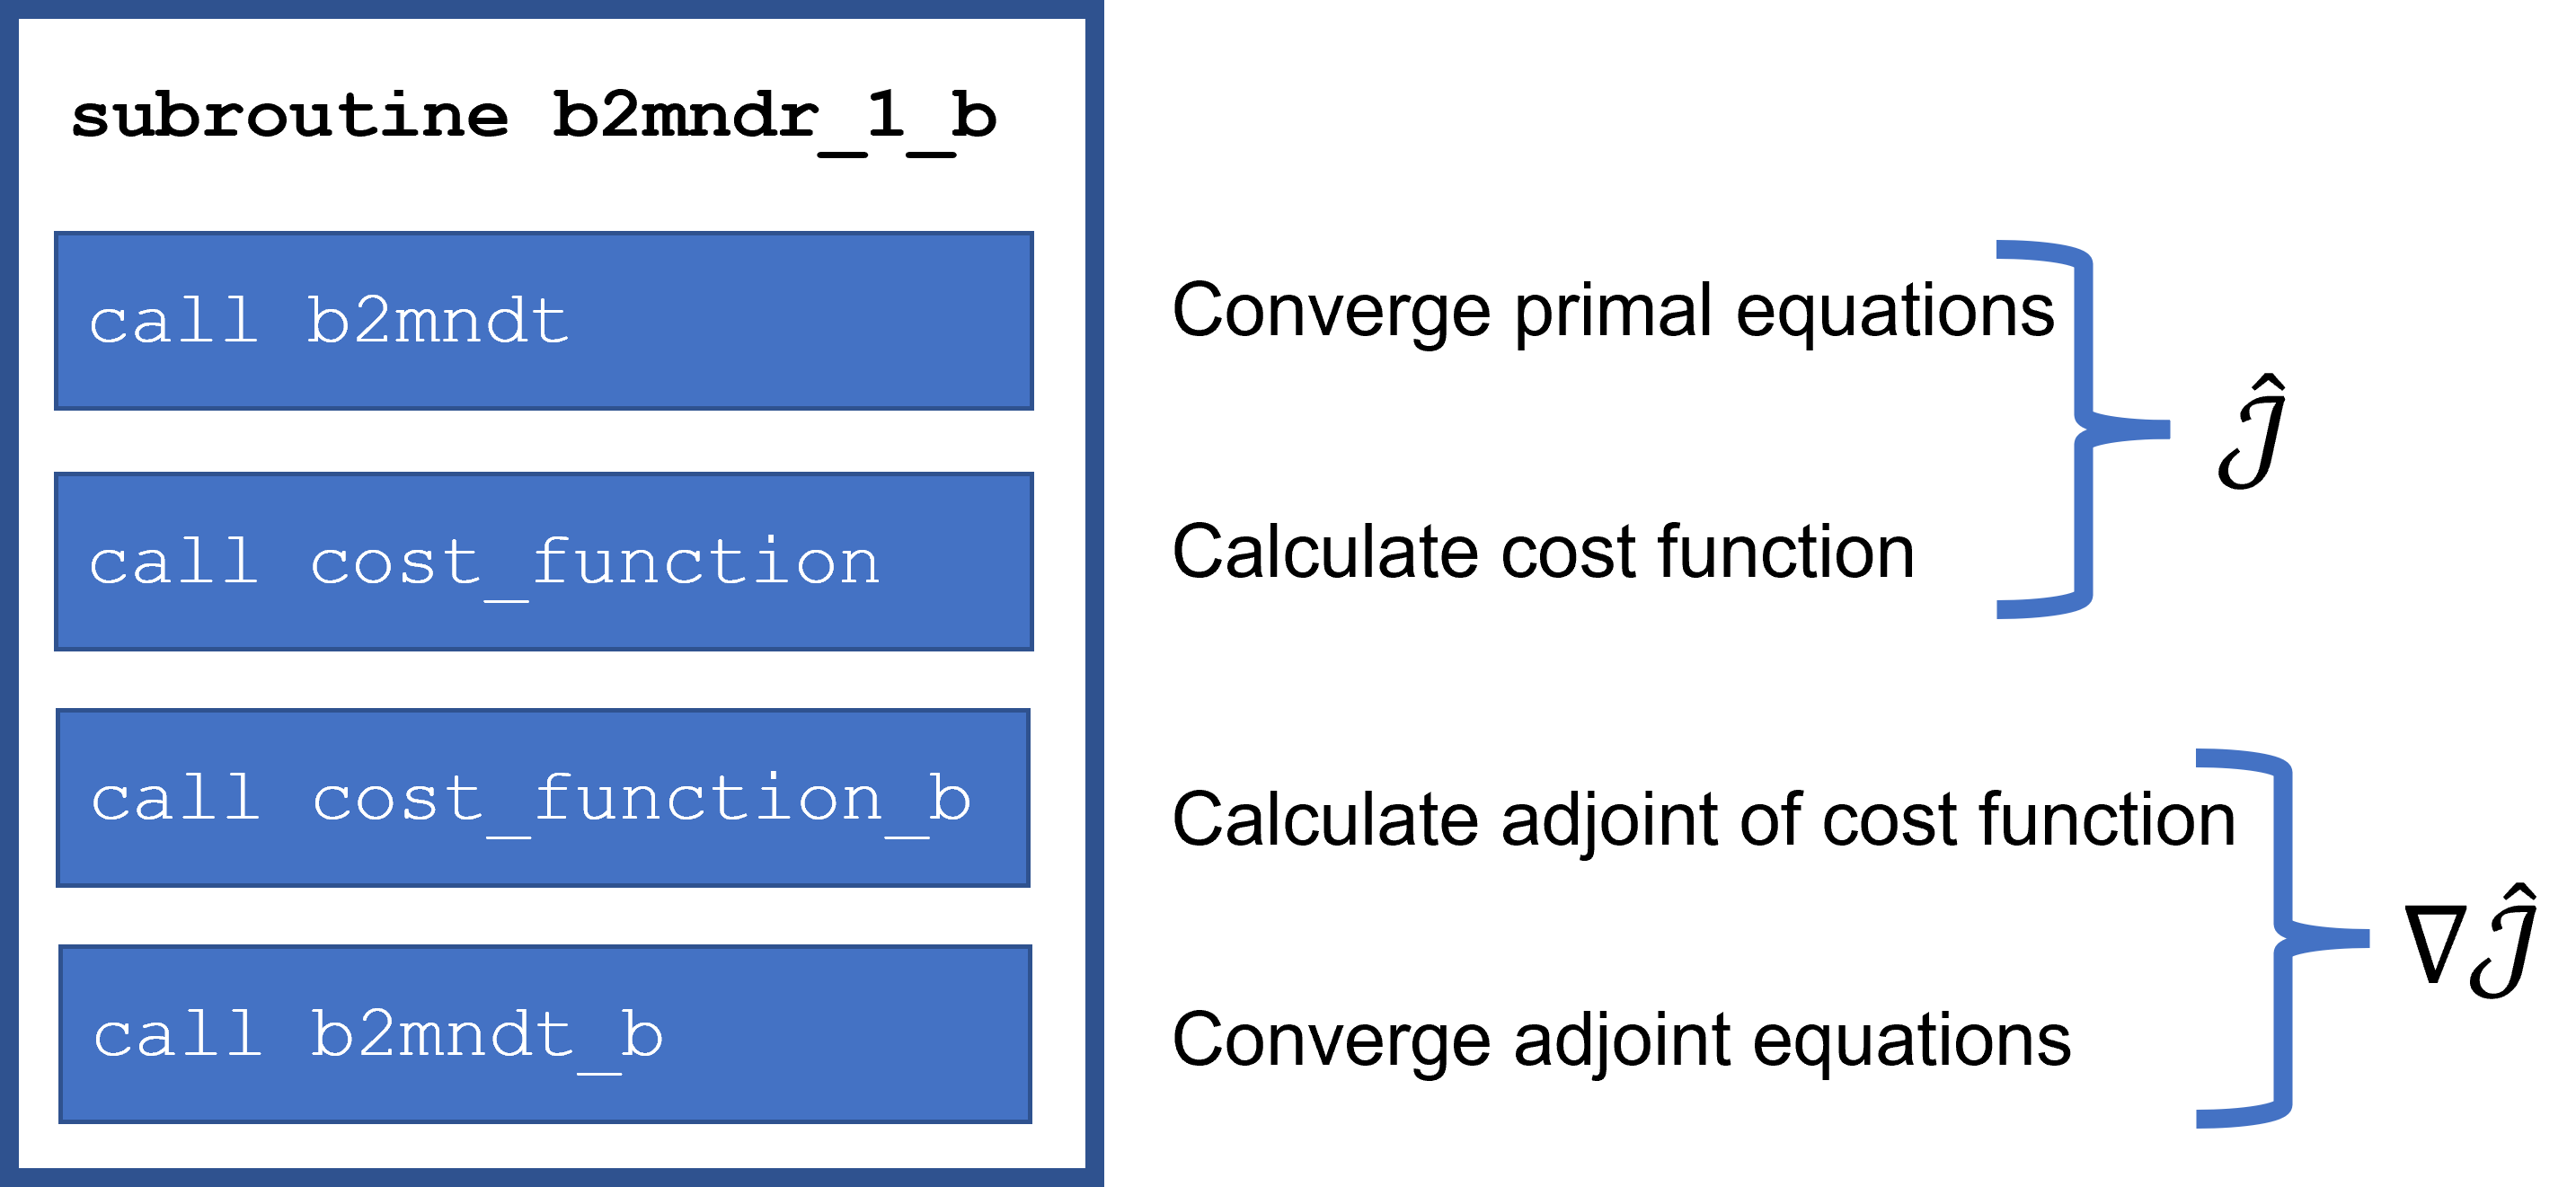
\includegraphics[width=120mm]{FiguresAD/adjoint_driver}
			\caption{Scheme of the adjoint AD main driver routine. \label{fig_adjoint}}
		\end{center}
	\end{figure}

	By default, running this version of the code will calculate the derivative of the FIRST cost function wrt all the default parameters indicated above.
	At each adjoint iteration it will print out in run.log the following information:
	\begin{itemize}
		\item GRADIENT ITERATION: current adjoint iteration
		\item GRADIENT MAX RES: current value of the maximum residual
	\end{itemize}
	It will also print the derivative of:
	\begin{itemize}
		\item {\tt parm\_dna(1)}: particle diffusion coefficient for species 1
		\item {\tt parm\_hce}:  electron heat diffusion coefficient
		\item {\tt parm\_hci(1)}: ion heat diffusion coefficient for species 1
		\item {\tt conpar(1,1,1)}: continuty BC for species 1 at boundary 1
		\item {\tt enepar(1,1)}: electron heat BC at boundary 1
		\item {\tt enipar(1,1)}: ion heat BC at boundary 1
		\item {\tt b2recyc(1,2)}: recycling coefficient for species 1 at stratum 2
	\end{itemize}

	To obtain such information simply do:\\
	{\\ \$ grep -i gradient run.log}\\

	At the end of the run it will eventually print the gradient of all the default parameters for species [0-1], boundaries [1-6], and strata [1-5]. If more printout is needed during or at the end of the run then {\tt b2mod\_driver\_diff.F90} and {\tt b2mod\_main\_diff.F90} need to be modified accordingly.


	The users for the moment can only monitor the progress of the derived quantities by inspecting the output produced by the code. In addition they can use the following script:
	\begin{description}
		\item[res\_adj] This script allows the user to plot the value of the calculated adjoint residual as per Eq.\ref{res}, as a function of the iterations
	\end{description}

	%%%%%%%%%%%%%%%%%%%%%%%%%%%%%%%%%%%%%%%%%%%%%%%%%%%%%%%%%%%%%%%%%
	\subsection{Comparing tangent and adjoint }
	%%%%%%%%%%%%%%%%%%%%%%%%%%%%%%%%%%%%%%%%%%%%%%%%%%%%%%%%%%%%%%%%%
	Tangent and adjoint derivatives should always be the same up to machine precision, i.e. $10^{-14}$ or near that, while comparisons with finite differences resulted in discrepancies of $\sim10^{-6}$ (depending on the perturbation size). This has been verified in the paper \cite{carlijcp}. There was however one case in which discrepancy between tangent, adjoint and finite differences was quite larger, order $10^{-3}$ or even higher. This was encountered when the total momentum equation was switched ON. The reason is the when this equation is used, then an extra velocity correction is applied through a function like
	\begin{equation}
		min(max(x,y),max(x,x+y),max(y,x+y)),
	\end{equation}
	which at convergence (i.e. when the corrections are zero), has a large gradient discontinuity. Is is therefor suggested to not use the total momentum equation for tangent/adjoint, or modify it to make it a smooth function.

	Additional non-smoothnesses are likely present in the code, which could potentially hamper the gradient's accuracy. Whenever these are found, they should be added to this section.

%%%%%%%%%%%%%%%%%%%%%%%%%%%%%%%%%%%%%%%%%%%%%%%%%%%%%%%%%%%%%%%%%
%%%%%%%%%%%%%%%%%%%%%%%%%%%%%%%%%%%%%%%%%%%%%%%%%%%%%%%%%%%%%%%%%
\section{Optimization}\label{sec:optimization}
%%%%%%%%%%%%%%%%%%%%%%%%%%%%%%%%%%%%%%%%%%%%%%%%%%%%%%%%%%%%%%%%%
%%%%%%%%%%%%%%%%%%%%%%%%%%%%%%%%%%%%%%%%%%%%%%%%%%%%%%%%%%%%%%%%%
The optimization framework will try to minimize the cost function $\hat{\mathcal{J}}(\theta)$ by adjusting some parameters $\theta$, subject to bound constraints on the $\theta$ variables themselves:
\begin{equation}\label{optim}
	\begin{array}{ll}
		\min\limits_{\theta} \hat{\mathcal{J}}(\theta) \\
		\mathrm{s.t.}~\theta_{L}\le\theta\le\theta_{U},
	\end{array}
\end{equation}
where $\theta_{L}$ and $\theta_{U}$ are the lower and upper bounds for $\theta$ respectively. Currently, no other nonlinear constraint is implemented.

The minimization is carried out by coupling the tangent or adjoint AD code to some optimization libraries, such as PETCs/TAO \cite{petsc1} or Ipopt \cite{ipopt}. What these optimizers do is to calculate the cost function and its gradient starting from an initial guess supplied by the user. Once the gradient is known, a suitable direction is computed along which the cost function decreases. This descent direction depends on the algorithm chosen (BFGS is the default, other possibilities include other quasi-Newton methods, steepest-descent, conjugate gradient, etc.). Subsequently, a so-called line-search is typically applied to find a step-length in the descent direction that guarantees convergence of the algorithm. Also here different choices are possible, the most common ones require the Armijo or the strong Wolfe condition. With PETCs/TAO it is possible to flexibly choose the descent direction type, the line search options, or even switch to trust region in place of line search methods. Users who like to know more regarding optimization methods are encouraged to read \cite{nocedal}.

A schematic view of the optimization process is available in Figure \ref{fig_optim} when tangent AD is employed for gradient computation. The initial guess $X0$ is fed to the tangent AD version of the main driver routine {\tt b2mndr\_1\_d}, which will compute the value of cost function and its gradient. If certain criteria regarding tolerances, computational time or iterations are met (see below), the optimization is stopped, otherwise the line search procedure is started and a new value for the parameters $\theta$ is computed and fed again to the main driver. Note that the line search will actually require one or more additional calls to the driver routines to evaluate the cost function and/or the gradient.

If adjoint AD is used for gradient calculation, then the driver routine {\tt b2mndr\_1\_d} in Figure \ref{fig_optim} is substituted by {\tt b2mndr\_1\_b} shown previously in Figure \ref{fig_adjoint}.

\begin{figure}[h]
	\begin{center}
		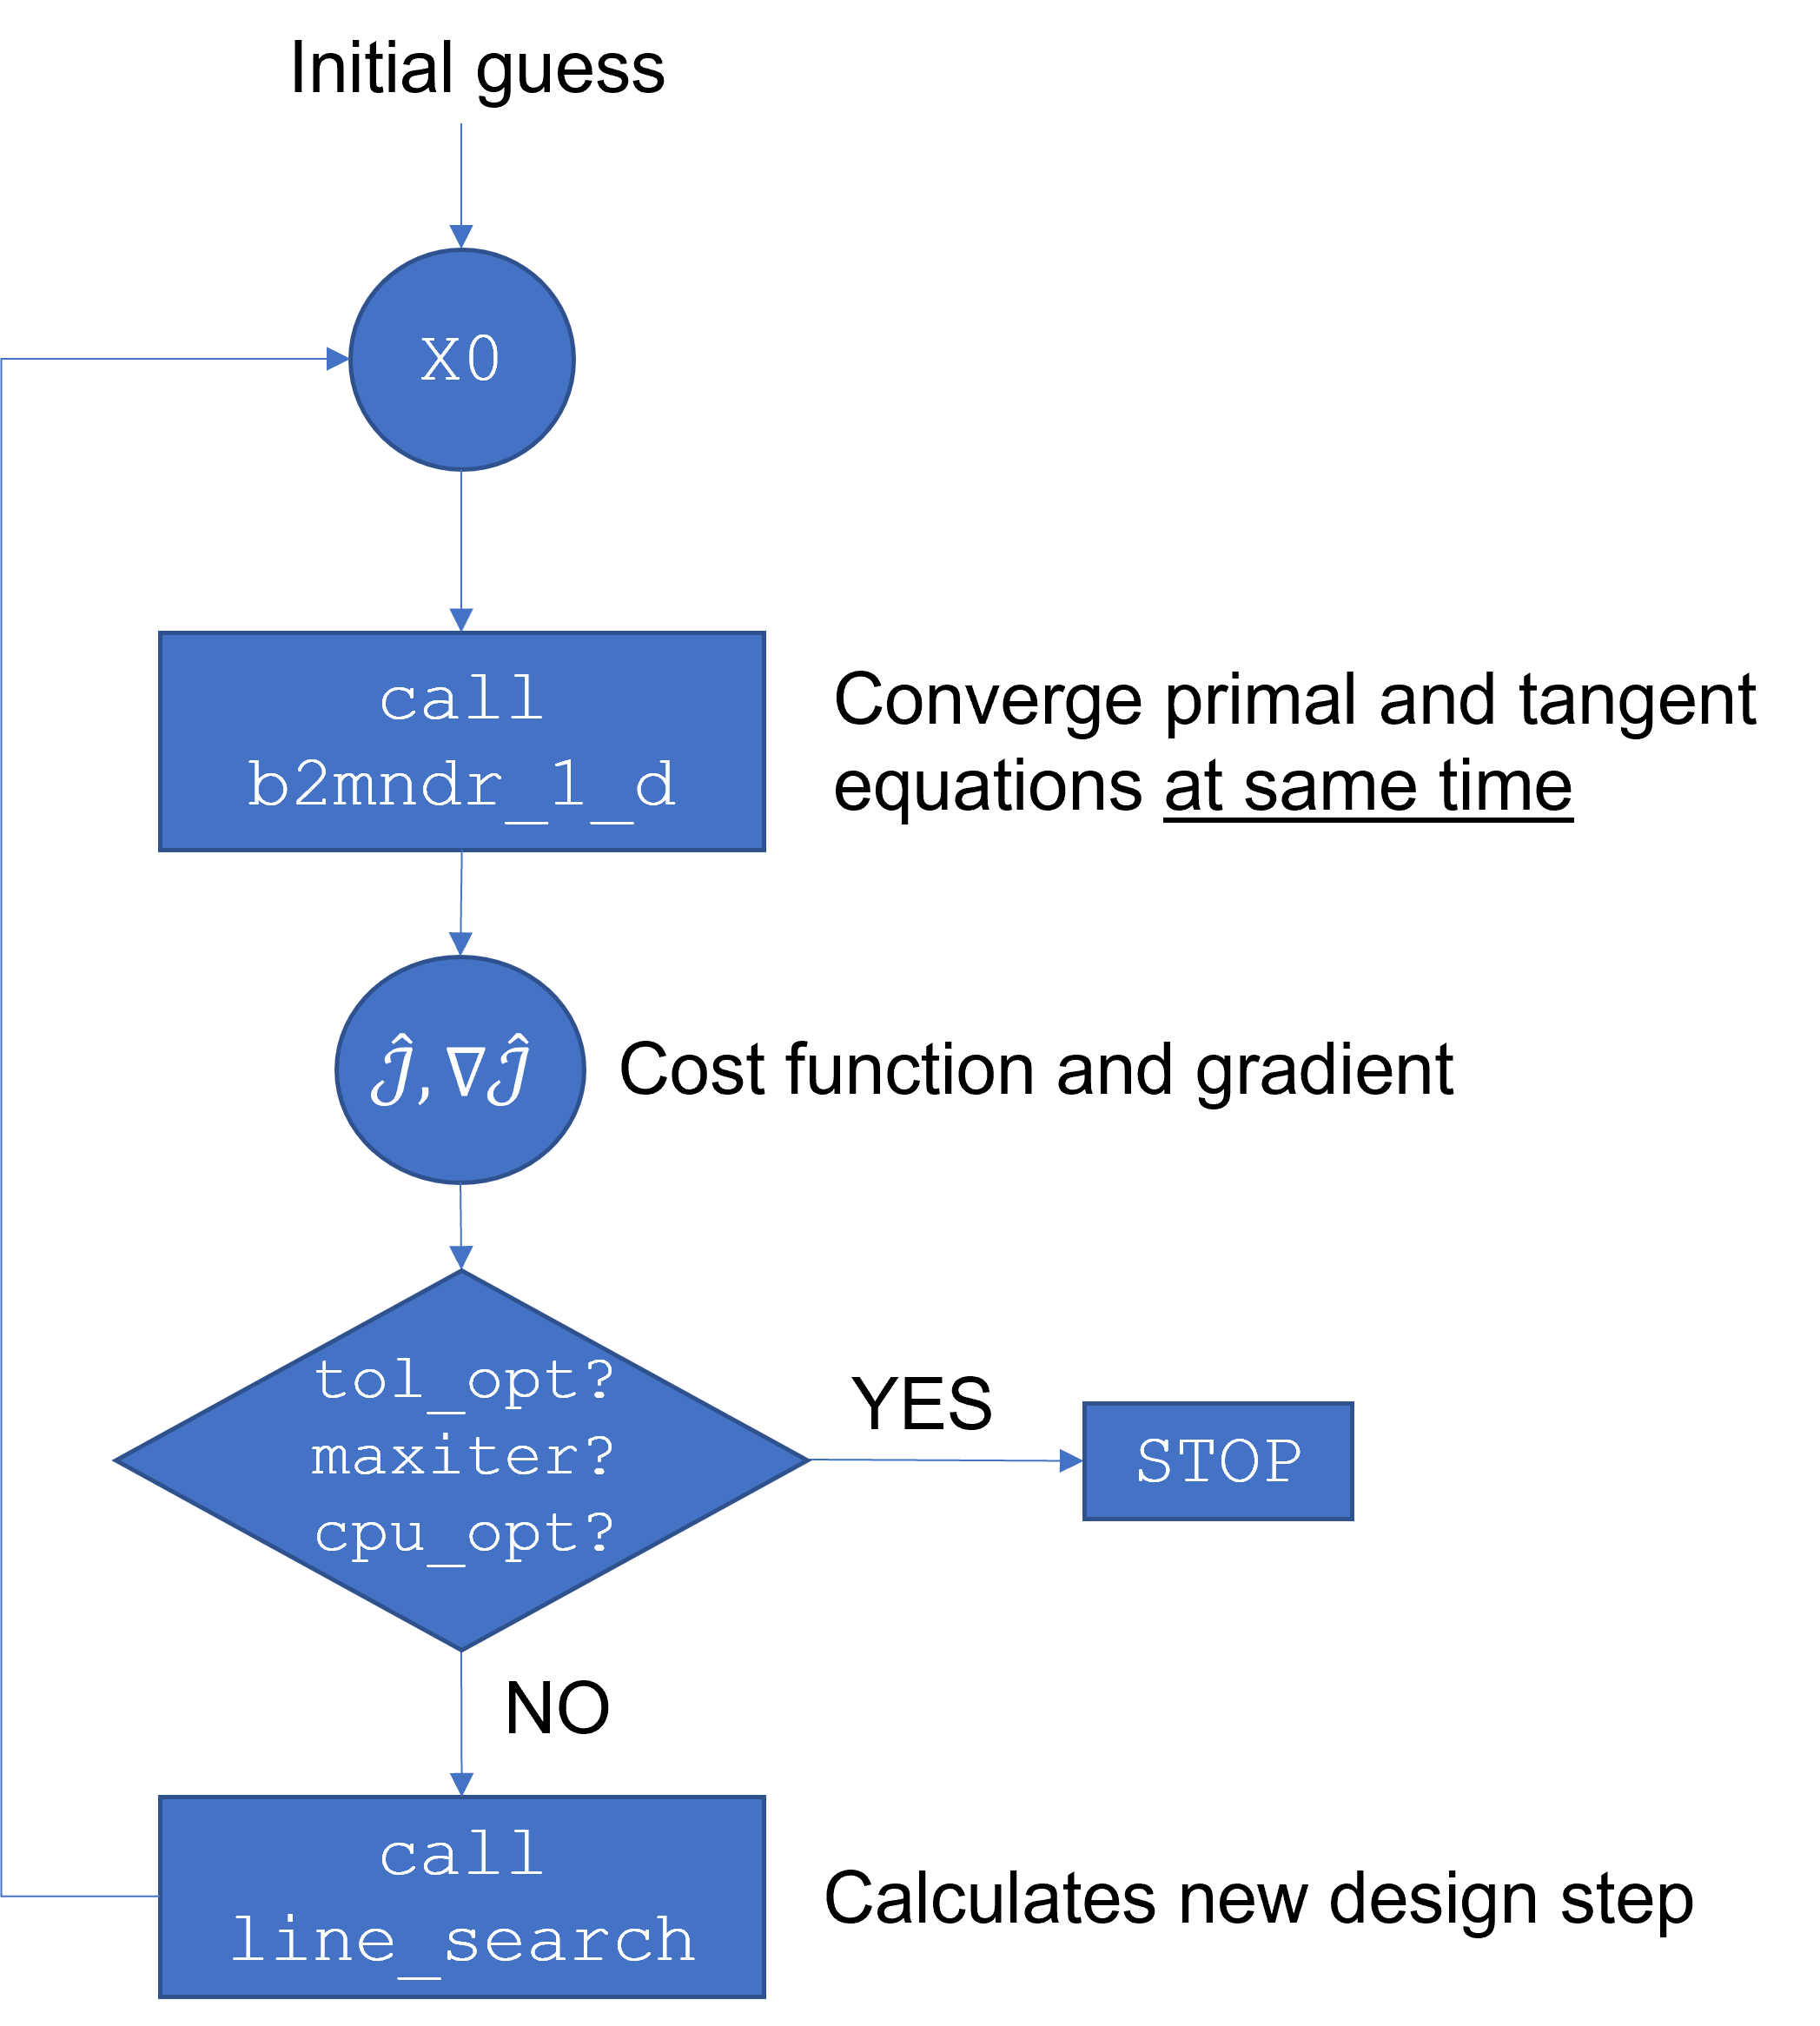
\includegraphics[width=120mm]{FiguresAD/optimization_scheme}
		\caption{Scheme of the tangent AD optimization. \label{fig_optim}}
	\end{center}
\end{figure}


Stopping criteria for the optimization:
\begin{itemize}
	\item zero-gradient (it means a stationary point / local minimum has been reached)
	\item maximum number of iterations reached
	\item maximum amount of CPU time
	\item tolerance met
\end{itemize}

For PETCs/TAO the tolerance is easily linked with optimization quantities like gradient and cost function, so that the optimization is stopped when the norm of the gradient is small enough $\left|\left |\nabla \hat{\mathcal{J}}\right|\right| \le \epsilon_a $, when the relative norm of the gradient is small enough $ \frac{\left|\left |\nabla \hat{\mathcal{J}}\right|\right|}{\left|\hat{\mathcal{J}}\right|} \le \epsilon_r $, or when the gradient has been sufficiently reduced wrt its value at the zeroth iteration $\frac{\left|\left |\nabla \hat{\mathcal{J}}\right|\right|} {\left|\left |\nabla \hat{\mathcal{J}}_0\right|\right|} \le \epsilon_t $. The various tolerances $\epsilon$ are set to the same default {\tt TOL\_OPT} (see b2.optimization.parameters in \ref{run_opt}), but with command line options they can be controlled separately.

	%%%%%%%%%%%%%%%%%%%%%%%%%%%%%%%%%%%%%%%%%%%%%%%%%%%%%%%%%%%%%%%%%
	\subsection{Compile optimization code}
	%%%%%%%%%%%%%%%%%%%%%%%%%%%%%%%%%%%%%%%%%%%%%%%%%%%%%%%%%%%%%%%%%
	In order to compile the optimization code, one must make sure that one of the optimization library currently tested with B2.5 is available, such as PETCs/TAO and Ipopt, either as a module to be loaded or as locally installed library from the user. Both PETCs/TAO and Ipopt are open source so the latter should always be feasible.

	For the local installation on the KU Leuven VSC cluster, for PETC/TAO to the following command line options to configure the installation were used:\\

	{\tt \$ ./configure {\tt-{}-with-mpi=0}} {\tt-{}-with-fc=ifort} {\tt-{}–with-cpp:/lib/cpp} {\tt-traditional} \\{\tt-{}-download-cmake=yes} {\tt-{}-download-superlu=yes} \\

	On other clusters a similar configuration could be used. It was in particular necessary to make sure that when loading the PETCs/TAO module or library the default compiler and compiler options of SOLPS were retained and not overwritten by those of the library.


	To compile the optimization version, for example with PETCs/TAO optimization library:\\
	{\tt \$ game listobj depend}\\
	{\tt \$ set\_tao}\\
	{\tt \$ gmake b25\_tgt b25\_adj}\\

	where {\tt SET\_TAO} allows to include extra compilation flags in the user's config files of B2.5. Alternatively, one can do the same with command {\tt SET\_IPOPT}. In both cases an additional executable named {\tt b2optim\_tao} or {\tt b2optim\_ipopt} is compiled in: \\
	{\tt B2.5/builds/standalone.}{\tt\${HOST\_NAME}}.{\tt\${COMPILER}}.{\tt[tgt-adj]}.\\

	%%%%%%%%%%%%%%%%%%%%%%%%%%%%%%%%%%%%%%%%%%%%%%%%%%%%%%%%%%%%%%%%%
	\subsection{Run an optimization}\label{run_opt}
	%%%%%%%%%%%%%%%%%%%%%%%%%%%%%%%%%%%%%%%%%%%%%%%%%%%%%%%%%%%%%%%%%
	After successful compilation, the optimization case can be setup. This requires a new file, {\tt b2.optimization.parameters}, which allows choosing which parameters to optimize, their starting guess, lower/upper bounds, as well as other optimization parameters. Additionally, one may need to adjust also {\tt b2.user.parameters} in case a MAP estimation takes place (see example below).

	Below is a description of the variables set in {\tt b2.optimization.parameters} within the {\tt OPTIMIZATION} namelist. An up-to-date list is also available in \ref{lis:b2cdcn}.

	\begin{description}
		\item[NNVAR]\index{NNVAR} {\tt integer}, number of optimization parameters $\theta$ (radially varying transport coefficients count as 1 as a whole) ({\tt ipar = 1, NNVAR}). ({\tt DEFAULT = 0}).

		\item[PARTYPE] \index{PARTYPE} {\tt integer array, length NNVAR}, indicates the type of optimization parameter $\theta$ for index {\tt ipar}. ({\tt DEFAULT = -1}). Available options are:
		\begin{description}
			\item[0] {\tt SIGMA}, standard deviation $\sigma_{q,l}$ in liklelihood function for Bayesian inference (one for each plasma quantity and location used). These must ALWAYS be the last parameters in the {\tt PARTYPE} vector!
			\item[1] {\tt parm\_dna} or {\tt tdata(:,:,1,:)}
			\item[2] {\tt parm\_dpa} or {\tt tdata(:,:,2,:)}
			\item[3] {\tt parm\_hci} or {\tt tdata(:,:,3,:)}
			\item[4] {\tt parm\_hce} or {\tt tdata(:,:,4,:)}
			\item[5] {\tt parm\_vla} or {\tt tdata(:,:,5,:)} (not yet tested!)
			\item[6] nothing yet (presumably y-component of vla?)
			\item[7] {\tt parm\_vsa} or {\tt tdata(:,:,7,:)}
			\item[8] {\tt parm\_sig} or {\tt tdata(:,:,8,:)}
			\item[9] {\tt parm\_alf} or {\tt tdata(:,:,9,:)}
			\item[10] {\tt enepar}
			\item[11] {\tt enipar}
			\item[12] {\tt conpar}
			\item[13] {\tt mompar}
			\item[14] {\tt potpar}
			\item[15] {\tt enkpar}
			\item[16] {\tt b2recyc}
			\item[17] {\tt b2tqna\_ballooning}
			\item[18] {\tt b2tqna\_ballooning\_rescale}
			\item[19] {\tt keps\_cd}
			\item[20] {\tt keps\_heat}
			\item[21] {\tt keps\_heat\_i}
			\item[22] {\tt keps\_sig}
			\item[23] {\tt keps\_alf}
			\item[24] {\tt keps\_visc}
			\item[25] {\tt keps\_dkt}
			\item[26] {\tt keps\_dzt}
			\item[27] {\tt b2sikt\_fac\_diss}
			\item[28] {\tt b2sikt\_fac\_diss\_core}
			\item[29] {\tt b2sikt\_fac\_sheath}
			\item[30] {\tt b2sikt\_fac\_sheath\_core}
			\item[30] {\tt keps\_shear}
			\item[30] {\tt b2tfhi\_fsigkt}
			\item[30] {\tt b2sikt\_fac\_vis\_RS}
			\item[30] {\tt b2tfhi\_fflokt}
			\item[30] {\tt b2tfhi\_fconkt}
			\item[30] {\tt b2tfhi\_fflozt}
			\item[30] {\tt b2tfhi\_fconzt}
			\item[30] {\tt b2tfhi\_fkt\_hie}
			\item[30] {\tt b2tfhe\_vis\_kt}
		\end{description}

		\item[SIGMA\_OPT] \index{SIGMA\_OPT} {\tt logical array, length NSIGMA}, for each sigma, specifies whether it is optimized or fixed. ({\tt DEFAULT = .true.}).

		\item[SPATIAL\_DEP] \index{SPATIAL\_DEP} {\tt logical array, length NNVAR}, for each optimization variables {\tt ipar}, specifies if radially varying coefficients are optimized.	Meaningful only for partype = 1 to 9. ({\tt DEFAULT = .false.}).

		\item[SPATIAL\_POINTS] \index{SPATIAL\_POINTS} {\tt integer array, length NNVAR}, number of spatial points optimized for parameter {\tt ipar} (should be the same as ndata in b2.transport.inputfile). The actual number of optimized variables (NPAR\_OPT) is then equal to the total number of spatial points + any other additional parameter. ({\tt DEFAULT = 0}).

		\item[PARIS] \index{PARIS} {\tt integer array, length NNVAR}, specifies the species of the optimization parameter {\tt ipar}. Only meaningful for {\tt partype} = [1-3,5,7,12,13,16]. ({\tt DEFAULT = 0}).

		\item[PARIB] \index{PARIB} {\tt integer array, length NNVAR}, specifies the boundary/strata of the optimization parameter {\tt ipar}. Only meaningful for {\tt partype} = [10-16]. ({\tt DEFAULT = 0}).

		\item[PAR\_RESCALE] \index{PAR\_RESCALE} {\tt real*8 array, length NPAR\_OPT}, coefficient to rescale optimization parameters (and their gradient). Note that the dimension is NPAR\_OPT, so it needs to be specified also for each spatial point in case of radially varying coefficients. ({\tt DEFAULT = 1.0}).

		\item[X0] \index{X0} {\tt real*8 array, length NPAR\_OPT}, initial guess for each optimization parameter. (p\_infty is a parameter currently set to 1e30). ({\tt DEFAULT = 10*p\_infty}).

		\item[XL] \index{XL} {\tt real*8 array, length NPAR\_OPT}, lower bound for each optimization parameter. ({\tt DEFAULT = -10*p\_infty}).

		\item[XU] \index{XU} {\tt real*8 array, length NPAR\_OPT}, upper bound for each optimization parameter. ({\tt DEFAULT = 10*p\_infty}).

		\item[CPU\_OPT] \index{CPU\_OPT} {\tt real*8}, maximum amount of CPU time in seconds after which the optimization is stopped. ({\tt DEFAULT = 0.0}).

		\item[MAXITER] \index{MAXITER} {\tt integer}, maximum number of optimization iterations. The maximum number of cost function evaluations is set to {\tt 2*MAXITER} to allow for line searches. Can be overridden with PETCs/Tao by using command line options for the optimization. ({\tt DEFAULT = 100}).

		\item[TOL\_OPT] \index{TOL\_OPT} {\tt real*8}, tolerance below which optimization is stopped. For PETCs/Tao it is used for the absolute gradient norm, the relative gradient norm, and the gradient reduction stopping criteria. Can be overridden with PETCs/Tao by using command line options for the optimization. ({\tt DEFAULT = 1.0e-7}).

		\item[HESSIAN\_APPROXIMATION] \index{HESSIAN\_APPROXIMATION} {\tt character*256}, type of Hessian approximation employed. Depends on optimization library. Possible values are currently: 'limited-memory' and 'exact'. When using the 'exact' option the steepest descent algorithm is used. ({\tt DEFAULT = 'limited-memory'}).

		\item[LIMITED\_MEMORY\_UPDATE\_TYPE] \index{LIMITED\_MEMORY\_UPDATE\_TYPE} {\tt character*256}, specifies which kind of Hessian approximation is employed if HESSIAN\_APPROXIMATION is set to 'limited-memory'. Can overridden with PETCs/Tao by using command line options for the optimization ({\tt DEFAULT = 'bfgs'}).

		\item[HESSIAN\_APPROXIMATION] \index{HESSIAN\_APPROXIMATION} {\tt character*256}, type of Hessian approximation employed. Depends on optimization library. Possible values are currently: 'limited-memory' and 'exact'. When using the 'exact' option the steepest descent algorithm is used. ({\tt DEFAULT = 'limited-memory'}).

		\item[NNCON] \index{NNCON} {\tt integer}, number of nonlinear constraints to impose. (not used for the moment) ({\tt DEFAULT = 0}).

		\item[GL] \index{GL} {\tt real*8 array, length NNCON}, lower bound for each nonlinear constraints. (not used for the moment). ({\tt DEFAULT = -10*p\_infty}).

		\item[GU] \index{GU} {\tt real*8 array, length RNNCON}, upper bound for each nonlinear constraints. (not used for the moment). ({\tt DEFAULT = 10*p\_infty}).

		\item[NNJAC] \index{NNJAC} {\tt integer}, number of non-zeros in Jacobian for the non-linear constraints. (not used for the moment). ({\tt DEFAULT = 0}).

		\item[JCOL] \index{JCOL} {\tt integer array, length NNJAC}, contains the column index of the non-zero element of the Jacobian for the non-linear constraints. (not used for the moment). ({\tt DEFAULT = 0}).

		\item[JROW] \index{JROW} {\tt integer array, length NNJAC}, contains the row index of the non-zero element of the Jacobian for the non-linear constraints. (not used for the moment). ({\tt DEFAULT = 0}).

		\item[JJ] \index{JJ} {\tt real*8 array, length NNJAC}, contains the value of the non-zero element of the Jacobian for the non-linear constraints. (not used for the moment). ({\tt DEFAULT = 0.0}).

	\end{description}


	Once the optimization case is ready, it can be started with the command:\\
	{\tt \$ set\_tao}\\
	{\tt \$ b2run -opt\_tgt > run.log}  OR {\tt \$ b2run -opt\_adj > run.log}\\

	Note that switches like {\tt b2mndr\_ntim} and {\tt b2mndr\_elapsed} will set the number of iterations or cpu time\textit{ for each single call} to {\tt b2mndr\_1\_[db]}. More tricky is the case of {\tt b2mndr\_etim}, which for now is suggested to be set to 0.0.

	Note additionally that {\tt b2mn\_d.F90} need not be modified to run the tangent optimization with a smaller/larger set of parameters (see \ref{sec:tanget_more})! One need only to specify them with b2.optimization.parameters.

	Finally, when optimization libraries like PETCs/TAO enable to modify options using command line arguments, the user can also do so by setting the environment variable:\\
	{\tt \$ setenv TAO\_OPT = "list-of-valid-options"}\\


	\textbf{Some suggestions:}
	\begin{itemize}
		\item scaling of the problem is quite important! therefore, aim at parameters which are in a similar range of order of magnitude, using {\tt par\_rescale};
		\item PETCs/TAO requires by default the strong Wolfe conditions for the line search, which may be too strict or be affected by gradient discontinuities. It may be better to require Armijo condition only with setting the option {\tt setenv TAO\_OPT = "-tao\_ls\_type armijo"};
		\item the BFGS method with PETCs/TAO seemed so far the most performing option, with Iptop and other PETCs/TAO methods more demanding.
	\end{itemize}

	%%%%%%%%%%%%%%%%%%%%%%%%%%%%%%%%%%%%%%%%%%%%%%%%%%%%%%%%%%%%%%%%%
	\subsection{Example of optimization setup}
	%%%%%%%%%%%%%%%%%%%%%%%%%%%%%%%%%%%%%%%%%%%%%%%%%%%%%%%%%%%%%%%%%
	\textbf{Regression cost function}\\
	For an estimation using a regression cost function as in the example in \ref{sec:cfexample}), one could think of optimizing particle and heat transport coefficients ($D_{\perp}$, $\chi_{\perp,i}$, and $\chi_{\perp,e}$), as well as the density BC for D+ ions at the core. In this case the {\tt b2.optimization.parameters} file could look like this:\\
	{\tt nnvar = 4,}\\
	{\tt partype =        1,  3,  4,                 12,}\\
	{\tt paris  =         1,  1,  0,                  1,}\\
	{\tt parib  =         3*0,                        1,}\\
	{\tt par\_rescale =    3*1.0,                   1.0e19,}\\
	{\tt x0 =              1.0,      1.0,     1.0,  1.00e19,}\\
	{\tt xl =              0.1,      0.1,     0.1,  0.5e19, }\\
	{\tt xu =             10.0,     15.0,    25.0,  1.5e19, } \\
	{\tt spatial\_dep =  F,F,F,}\\
	{\tt spatial\_points = 0,0,0,}\\
	{\tt maxiter = 20,}\\
	{\tt tol\_opt = 1.0e-4,}\\
	{\tt cpu\_opt = 255000.0,}\\
	{\tt hessian\_approximation = limited-memory,}\\
	{\tt limited\_memory\_update\_type = bfgs,}\\
	{\tt nncon = 1,}\\
	{\tt nnjac = 1,}\\
	{\tt jcol = 1,}\\
	{\tt jrow = 1,}\\
	{\tt jj = 0.0,}\\

	The eplanation is as follows: we optimize four parameters, thus {\tt nnvar=4}; these four parameters are, in order:
	\begin{description}
		\item $D_{\perp}$ for D+ ions ({\tt parm\_dna(1)}). Thus {\tt par\_type(1)=1}, for species 1, thus {\tt par\_is(1)=1}. {\tt par\_ib(1)} does not matter and is set to zero
		\item $\chi_{\perp,i}$ for D+ ions ({\tt parm\_hci(1)}). Thus {\tt par\_type(2)=3}, for species 1, thus {\tt par\_is(2)=1}. {\tt par\_ib(2)} does not matter and is set to zero
		\item $\chi_{\perp,e}$ ({\tt parm\_hce}). Thus {\tt par\_type(3)=4}. {\tt par\_ib(3)} and {\tt par\_is(3)} do not matter
		\item continuity BC at the core for D+ ({\tt bccon(1,1,1)}). Thus {\tt par\_type(4) = 12}), for species 1, thus {\tt par\_is(4)=1}, and for core boundary (in this case 1), thus {\tt par\_ib(4)=1}
	\end{description}
	Moreover, the starting guess for each of the transport coefficients is 1.0, while for the density BC this is $10^{19} m^{-3}$. As such, {\tt x0 = 1.0, 1.0, 1.0, 1.0e19} (and {\tt xl, xu} are defined in a similar way).

	Since the density BC has a quite different order of magnitude, which will considerably hamper the optimization process, it is better to rescale this parameter and the related gradient component such that it falls in the vicinity of the order of magnitude of the other parameters. Therefore, {\tt par\_rescale(4) = 1.0e19}.

	There is no radial dependent transport coefficient in this case, so we set {\tt spatial\_dep = F,F,F} and {\tt spatial\_points = 0,0,0}.

	Next, we set as stopping criteria a maximum number of 20 optimization iterations with {\tt maxiter=20}, a minimum tolerance of $10^{-4}$ with {\tt tol\_opt = 1e-4}, and maximum of about 71 hours of cpu time for the optimization with {\tt cpu\_opt = 255000.0}.

	The last parameters could be omitted in a standard optimization with PETCs/TAO BFGS and without nonlinear constraints, while they should be specified for Ipopt, as in there a 'hard-coded' trivial constraint needs to be specified (automatically done).\\

	\textbf{Radially dependent coefficients}\\
	If one wants to optimize radially dependent transport coefficients the setup above can be modified according to:\\
	{\tt par\_rescale =    6*1.0,    6*1.0.   6*1.0,          1.0e19,}\\
	{\tt x0 =              6*1.0,    6*1.0,   6*1.0,  1.00e19,}\\
	{\tt xl =              6*0.1,    6*0.1,   6*0.1,  0.5e19, }\\
	{\tt xu =             6*10.0,   6*15.0,   6*25.0,  1.5e19, } \\
	{\tt spatial\_dep =  T,T,T,}\\
	{\tt spatial\_points = 6,6,6,}\\

	The major difference wrt the previous example is that for each of the transport coefficients we now specify that there are 6 spatial points to be optimized ({\tt spatial\_dep=T,T,T} and {\tt spatial\_points=6,6,6}). Accordingly, we need to specify {\tt per\_rescale, x0, xl, xu} for each of these spatial points, therefore the additional {\tt 6*} if front of the values for {\tt part\_type(1:3)}.

	Note that the other optimization parameters don't need to change!

	Finally, one must be careful to have {\tt 'b2tqna\_inputfile'} set to {\tt '1'} and that in {\tt b2.transport.inputfile} the coefficients for {\tt kind\_coeff=1,3,4} are specified in 6 radial points.

	NOTE: the optimization will adapt the value of the transport coefficients at these radial locations, but will not `move' such locations!\\


	\textbf{MAP cost function}\\
	If the user is instead interested in a Bayesian MAP estimation, with a cost function again similar to the example above \ref{sec:cfexample}), the optimization setup needs to change, as well as the {\tt b2.user.parameters} file. Starting from the former, the b2.optimization.parameters file will read:\\
	{\tt nnvar = 9,}\\
	{\tt partype =        1,  3,  4,                 12, 5*0,}\\
	{\tt paris  =         1,  1,  0,                  1, 5*0,}\\
	{\tt parib  =         3*0,                        1, 5*0,}\\
	{\tt par\_rescale =    3*1.0,                   1.0e19, 5*1.0,}\\
	{\tt x0 =              1.0,      1.0,     1.0,  1.00e19,5*1.0,}\\
	{\tt xl =              0.1,      0.1,     0.1,  0.5e19, 5*1.0e-2,}\\
	{\tt xu =             10.0,     15.0,    25.0,  1.5e19, 5*10.0,} \\
	{\tt sigma\_opt = T,T,T,T,T,} \\
	{\tt spatial\_dep =  F,F,F,}\\
	{\tt spatial\_points = 0,0,0,}\\
	{\tt maxiter = 20,}\\
	{\tt tol\_opt = 1.0e-4,}\\
	{\tt cpu\_opt = 255000.0,}\\
	{\tt hessian\_approximation = limited-memory,}\\
	{\tt limited\_memory\_update\_type = bfgs,}\\
	{\tt nncon = 1,}\\
	{\tt nnjac = 1,}\\
	{\tt jcol = 1,}\\
	{\tt jrow = 1,}\\
	{\tt jj = 0.0,}\\

	While for optimization parameters 1 to 4 the same comments as in the first example optimization setup hold, we also added 5 extra variables, which refer to the {\tt SIGMA}'s in the likelihood function we also want to estimate. They are defined with {\tt partype(5:9) = 0}, no species or boundary needs to be specified for them ({\tt paris(5:9) = pairb(5:9) = 0}), and their initial value is set to 1.0. The rescaling and lower/upper bounds are also specified. Finally, one additional variable is employed now, {\tt SIGMA\_OPT = T,T,T,T,T,} which essentially makes that all 5 sigma values are optimized.

	If one already knows a priori the value of one of those sigmas, e.g. that of the ion temperature at the OMP ({\tt icf = 4}), then the \textit{third} value of {\tt SIMGA\_OPT} should be `F'.

	When looking at the {\tt b2.user.parameters} file, this is adjusted as:\\
	{\tt NCF = 6}\\
	{\tt CFTYPE = 6, 1, 2, 3, 1, 2}\\
	{\tt CFSTART = 2, 0, 0, 0, -34, -34,}\\
	{\tt CFEND =   6, 0,  0, 0, -34, -34,}\\
	{\tt CFDEF =   0, 1,  1,  1, 2, 2,}\\
	{\tt NSIGMA = 5,}\\
	{\tt SIGMA =  0.1, 0.1, 0.1, 0.2, 5,}\\
	{\tt SCALE\_SIGMA = T, T, T, F, F,}\\
	{\tt PRIOR\_TYPE = 4*0, 1, 1, 1, 0, 0,}\\
	{\tt PRIOR\_PAR(1,1) = 4*0.0, 0.0, 0.0, 0.0,}\\
	{\tt PRIOR\_PAR(1,2) = 4*0.0, 10.0, 10.0, 10.0,}\\
	{\tt PRIOR\_RANGE(1,1) = 4*1.0e-5, 1.0e-5, 1.0e-5, 1.0e-5, 1.0e-5, 1.0e-5,}\\

	where we have added 4 extra entries at the beginning of the arrays {\tt PRIOR\_TYPE},  {\tt PRIOR\_PAR}, and {\tt PRIOR\_RANGE}. The reasoning is that now the prior must include ALL the optimization parameters, not only the sigmas, in the order they are specified in {\tt b2.optimization.parameters}. As such {\tt PRIOR\_TYPE(1:4)} refer in this case to the prior for {\tt PARTYPE(1:4) = 1,3,4,12}, while {\tt PRIOR\_TYPE(5:9)} refer to {\tt PARTYPE(5:9) = 5*0}, i.e. the sigmas.

	In this specific case we used a uniform prior for the first four optimization parameters, while for the sigmas the same as in the example cost function is retained.

	Note that the prior range may be superfluous if a lower/upper bound for optimization parameters and sigmas is used, and vice versa.
